\documentclass[final]{beamer}

% ====================
% Packages
% ====================

\usepackage[T1]{fontenc}
\usepackage{lmodern}
\usepackage[orientation=portrait,size=a2,scale=1.15]{beamerposter}
\usepackage{multicol}
%\usepackage{bibtex}
\usetheme{gemini}
\usecolortheme{nott}
\usepackage{graphicx}
\usepackage{booktabs}
\usepackage{tikz}
\usepackage{csquotes}
\usepackage{pgfplots}
\pgfplotsset{compat=1.14}
\usepackage{anyfontsize}
\usepackage{lipsum}
\usepackage{bookmark}
\usepackage[brazil]{babel}
\usepackage[citestyle=alphabetic,bibstyle=authortitle,backend=biber]{biblatex}
\addbibresource{referencias.bib}

% ====================
% Lengths
% ====================

\newlength{\sepwidth}
\newlength{\colwidth}
\setlength{\sepwidth}{0.025\paperwidth}  % Largura da separação entre as colunas
\setlength{\colwidth}{0.45\paperwidth}    % Largura das colunas (ajustada para 2 colunas)

\newcommand{\separatorcolumn}{\begin{column}{\sepwidth}\end{column}}  % Comando para criar uma coluna separadora

% ====================
% Boxes around the topics
% ====================

\definecolor{color1}{RGB}{160,95,179} % Roxo claro

\setbeamercolor{block title}{bg=color1, fg=white}  % Título do bloco com fundo roxo e texto branco

% ====================
% Title
% ====================
\title{{\fontsize{35}{35}\selectfont Aplicação de Krigagem Ordinária em Dados
Meteorológicos do Rio Grande do Sul}}

\author{{\fontsize{19}{19}\selectfont 
Pedro Dresseno John \inst{1} \and 
Yuri Dessimon \inst{1} \and 
Márcia Helena Barbian \inst{1,2}}\\[1em]} % espaço extra autores → instituição

\institute[shortinst]{
  {\fontsize{16}{16}\selectfont
   \inst{1} Departamento de Estatística, UFRGS \samelineand
   \inst{2} Programa de Pós-Graduação em Estatística, UFRGS
   \inst{1} \texttt{johnpd4@gmail.com} \samelineand
   \inst{1} \texttt{yuridessimon@gmail.com} \samelineand
   \inst{1,2} \texttt{mhbarbian@gmail.com}
  }
}

% \author{{\fontsize{12}{12}\selectfont 
% johnpd4@gmail.com \and 
% yuridessimon@gmail.com \and 
% Márcia Helena Barbian \inst{1,2}}\\[1em]} % espaço extra autores → instituição


% \institute[shortinst]{{\fontsize{16}{16}\selectfont \inst{1} Universidade Federal do Rio Grande do Sul }}
% \author{{\fontsize{19}{19}\selectfont Pedro Dresseno John \inst{1} \and Yuri Dessimon \inst{1} \and Márcia Helena Barbian \inst{1,2}}\\[1.2em]}

% \institute[shortinst]{{\fontsize{15}{15}\selectfont \inst{1} Departamento de Estatística, UFRGS\\ \inst{2} Programa de Pós-Graduação em Estatística, UFRGS}}


% \title{{\fontsize{35}{35}\selectfont Aplicação de Krigagem Ordinária em Dados
% Meteorológicos do Rio Grande do Sul}}
% \author{{\fontsize{20}{20}\selectfont Pedro Dresseno John \inst{1} \and Yuri Dessimon \inst{1} \and Márcia Helena Barbian \inst{1,2}}}

% \institute[shortinst]{{\fontsize{16}{16}\selectfont \inst{1}  johnpd4@gmail.com \samelineand \inst{2} Departamento de Estatística, UFRGS - yuridessimon@gmail.com \samelineand \inst{3} Programa de Pós-Graduação em Estatística - UFRGS - mhbarbian@gmail.com }}

% ====================
% Logo (optional)
% ====================

\logoleft{\vspace{-1cm}\hspace{1cm}
\includegraphics[height=5cm]{./img/logos/logo-ss.png}}  % Reduzindo o espaço superior
\logoright{\vspace{0.5cm}
\includegraphics[height=5cm]{./img/logos/logo2.png}\hspace{1cm}}



\usetikzlibrary{calc}
\makeatletter
\AddToHook{shipout/foreground}{%
  \begin{tikzpicture}[remember picture,overlay]
       % ===================================================
    % DUAS LINHAS HORIZONTAIS (configuráveis)
    % Linha 1
    \draw[line width=15pt, color=color1] 
      ($(current page.north west)+(1cm,-0.5cm)$) -- ++(39.9cm,0);

    % Linha 2 (abaixo da primeira, distância definida pelo "-10cm")
    \draw[line width=15pt, color=color1] 
      ($(current page.north west)+(1cm,-6.2cm)$) -- ++(39.9cm,0);
    % ===================================================

  \end{tikzpicture}%
}
\makeatother

% ====================
% Body
% ====================



\begin{document}

\begin{frame}[t]
\begin{columns}[t]
\separatorcolumn  % Coluna separadora (espaço entre as colunas)

% Primeira coluna
\begin{column}{\colwidth}
  

\begin{beamercolorbox}[wd=\colwidth, sep=6pt, leftskip=6pt, rightskip=6pt]{block title}
 \fontsize{20}{22}\selectfont \centering{\textbf{Introdução}}
\end{beamercolorbox}



\begin{beamercolorbox}[wd=\colwidth, sep=2pt, leftskip=2pt, rightskip=2pt]{block body}
  \vspace{-2pt} % reduz espaço extra
  %A análise de dados espaciais com o modelo estatístico clássico normalmente define as médias como regressão linear das covariáveis e um processo gaussiano como modelo de covariância como a dependência espacial.
  \justifying{
    \hspace{1 cm}
    Eventos meteorológicos extremos são cada vez mais comuns, assim para garantir a segurança da população torna-se cada vez mais necessário ter modelos mais precisos, que possam informar política pública.
    Um método que permite tais previsões é o da Krigagem, uma técnica de interpolação geoestatística usada para estimar valores de uma variável em locais não observados baseados em locais amostrados.
    A aplicação de tal técnica permite melhores previsões de vários fenômenos naturais como a chuva e temperatura que são importantes indicadores de eventos extremos.
    %\textcolor{red}{explicar um pouco mais,sobre problemas meteriológicos... que é importante estimar a quantidade de chuvas...}
    O objetivo desse trabalho é estimar a distribuição espacial da precipitação e temperatura no estado do Rio Grande do Sul no mês de fevereiro de 2025, para isso serão considerados dados meteorológicos coletados em 40 centros de monitoramento espalhados no  estado \cite{INMET_2025}.

}  
  
  \vspace{4pt}
\end{beamercolorbox}


%%%%%%%%%%%%%%%%%%%%%%%%%%%%%%%%%%%%%%%%%%%%%%%%%%%%%%%%%%%%%%%%%%%%%%%
% \begin{beamercolorbox}[wd=\colwidth, sep=6pt, leftskip=6pt, rightskip=6pt]{block title}
%  \fontsize{20}{22}\selectfont \centering{\textbf{Objetivo}}
% \end{beamercolorbox}
% \begin{beamercolorbox}[wd=\colwidth, sep=2pt, leftskip=2pt, rightskip=2pt]{block body}
%   \vspace{-2pt} % reduz espaço extra
%     \justifying{
% \hspace{1 cm} 

% }
%   \vspace{4pt}
% \end{beamercolorbox}
\begin{beamercolorbox}[wd=\colwidth, sep=6pt, leftskip=6pt, rightskip=6pt]{block title}
 \fontsize{18}{20}\selectfont \centering{\textbf{Meotodologia}}
\end{beamercolorbox}
\begin{beamercolorbox}[wd=\colwidth, sep=2pt, leftskip=2pt, rightskip=2pt]{block body}
  \vspace{-2pt} % reduz espaço extra

\justifying{ \hspace{1 cm} Para a estimativa da precipitação e da temperatura será utilizado o modelo geoestatístico tal que a variável de interesse \( Z(s) \) na localização \( s \in D \subset \mathbb{R}^2 \) é considerada como a realização do seguinte processo estocástico \cite{cressie2015statistics}: }


                \begin{equation}\label{eqn1_normal}
                Z(s) = \mu + \varepsilon(s),
                \end{equation}

            \hspace{1 cm} - $\mu$ média constante desconhecida; 
               
           \hspace{1 cm} - \( \varepsilon(s) \sim \mathcal{N}(0, C(h)) \) é um processo estacionário com esperança zero e função de covariância 
            \( C(h) = \text{Cov}(Z(s), Z(s+h)) \)            
            que é  dependente da distância \( h \). 

             \vspace{0.5cm}
        \justifying{
             \hspace{0.5cm} Sob essas condições, utilizou-se a krigagem ordinária, um estimador linear e não viciado definido pela Equação: \ref{eqn2_krig}: }
                \begin{equation}\label{eqn2_krig}
                \hat{Z}(s_0) = \sum_{i=1}^n \lambda_i Z(s_i),
                \end{equation}
                
          \hspace{1 cm}- $\hat{Z}(s_0)$ é o valor predito na localização $s_0$;

          \hspace{1 cm}- $Z(s_i)$ representa o valor observado da variável no local $s_i$;
        
          \hspace{1 cm}- $\lambda_i$ é o peso atribuído ao valor observado $Z(s_i)$.
            
           
    % \textcolor{red}{coloca os itens do modelo como topicos...
    % mu é isso, epsilon é isso, com media tal e covariancia tal....}           


\end{beamercolorbox}
%%%%%%%%%%%%%%%%%%%%%%%%%%%%%%%%%%%%%%%%%%%%%%%%%%%%%%%%%%%%%%%%%%%%%%%
%%%%%%%%%%%%%%%%%%%%%%%%%%%%%%%%%%%%%%%%%%%%%%%%%%%%%%%%%%%%%%%%%%%%%%%
\begin{beamercolorbox}[wd=\colwidth, sep=6pt, leftskip=6pt, rightskip=6pt]{block title}
 \fontsize{18}{20}\selectfont \centering{\textbf{Semivariograma}}
\end{beamercolorbox}
\begin{beamercolorbox}[wd=\colwidth, sep=2pt, leftskip=2pt, rightskip=2pt]{block body}
  \vspace{-2pt} % reduz espaço extra

\justifying{
                \hspace{1 cm} Nesse modelo é importante definir a função do semivariograma \( \hat{\gamma}(h) \),  que indicará a estrutura da função de covariância $C(h)$, que descreve a dependência espacial do processo. Uma forma de estimar o semivariograma não parametricamente é através da Equação

                \begin{equation}\label{eq:Variograma}
                   \hat{\gamma}(h) = \frac{1}{2 N(h)} \sum_{i=1}^{N(h)} \left( Z(s_i) - Z(s_i + h) \right)^2.
                \end{equation}
        
        
        \hspace{1 cm}- $N(h)$ é o número de pares de dados que estão separados pela distância $h$.
        %\item 
           }

\begin{figure}
    \centering
    \label{fig:3}
    
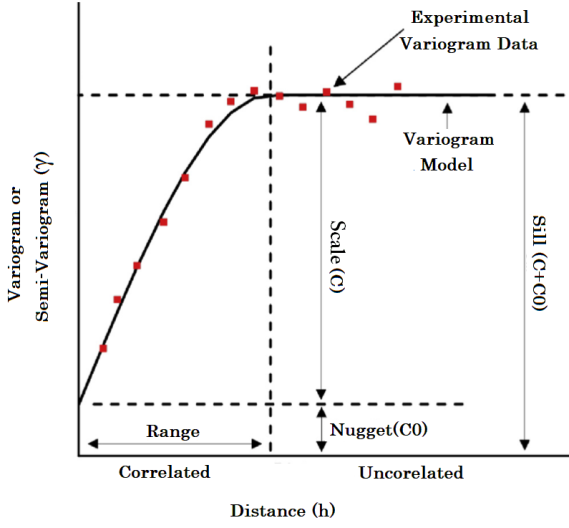
\includegraphics[width=15cm, height=10cm]{img/krig_ord/variogram.png}
    \caption{Parâmetros de um variograma e/ou semi variograma  Fonte: Bagheri Bodaghabadi (2018). \cite{bagheri2018necessarily}}
    \label{fig:variogram}
\end{figure}


           
\end{beamercolorbox}


\hspace{1 cm} Para o cálculo do variograma foi utilizada a função \textbf{VGM} e para krigagem foi utilizada a função \textbf{krige}, ambas do pacote \textit{gstat} \cite{gstat2}. A Figura 2 apresenta duas estimativas da precipitação para uma grade regular no RS usando modelos com variogramas de dois ângulos distintos.

Para a confecção das imagens da Figura 2 foi utilizado o pacote \textit{Leaflet}\cite{leaflet}. 

\begin{figure}
  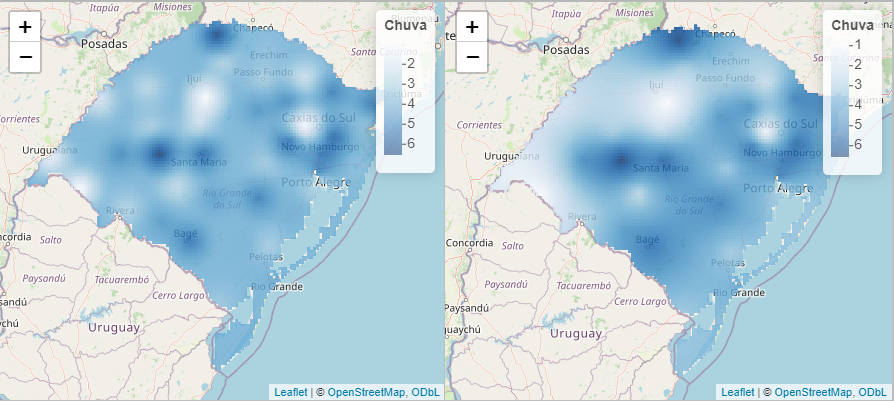
\includegraphics[width=0.9\textwidth]{./img/krig_ord/krig_all_angles2.png}
    \begin{center}
    \caption{\justifying{Diferente estimativas da precipitação, considerando uma diferentes ângulos para a função de covariância isotrópica. Fonte: Do autor}}
  \end{center}
  \label{fig:2}  
\end{figure}

\vspace{-1.5em}


\end{column}

\separatorcolumn  % Coluna separadora

% Segunda coluna

\begin{column}{\colwidth}

O uso de ângulos distintos é importante pois vários fenômenos físicos que acontecem no espaço são anisotrópicos, isso é temos diferentes relações entre a variável e a distância do ponto dependendo da direção em que estamos olhando. Na direita vemos a estimativa que faz uso do variograma com ângulo de 135 graus, enquato, na direita, temos a predição considerando um ângulo de 90 graus. A função de covariância escolhida pela função \textit{fit.variogram} do pacote \textit{gstat}, foi a função esférica para ambos os casos, e os parâmetros do modelo foram estimados numéricamente pela mesma função.

\vspace{0cm}
  \begin{beamercolorbox}[wd=\colwidth, sep=6pt, leftskip=6pt, rightskip=6pt]{block title}
 \fontsize{20}{22}\selectfont \centering{\textbf{Resultados}}
\end{beamercolorbox}
\begin{beamercolorbox}[wd=\colwidth, sep=2pt, leftskip=2pt, rightskip=2pt]{block body}
  \vspace{-2pt} % reduz espaço extra
\justifying{


 \hspace{1 cm} A Figura 3 apresenta a distribuição espacial estimada da precipitação, temperatura, vento e umidade no estado do Rio Grande do Sul. Observa-se um padrão espacial, com maiores valores de precipitação concentrados à esquerda da lagoa dos patos, enquanto as temperaturas mais elevadas são verificadas nas regiões próximas a Porto Alegre e noroeste do estado. Os modelos do vento e umidade tiveram interpolações que apenas diferem da média imediatamente na região próxima de uma estação. Melhores resultados para tais variáveis poderiam ser encontrados com algoritmos mais robustos de estimação de parâmetros, como o método da máxima verossimilhança.
%\textcolor{red}{no outro tu fala de anisotropia e aqui nao fala nada, comenta que só foi usado um angulo para estimar... de novo... isso é baseado em um modelo aproximado pela estimação nao parametrica ou tu usou o estimador nao parametrico da covariancia pra fzer a krigagem???}
}
  \vspace{0.7cm}
  
\begin{figure}[h!]  
\begin{center}
    
        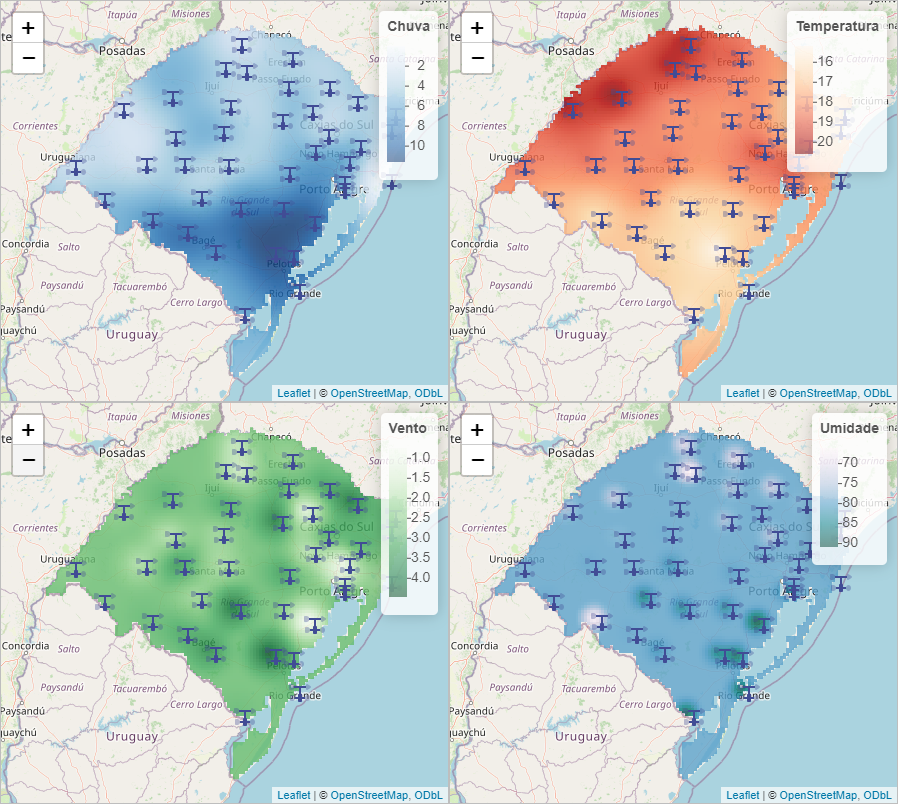
\includegraphics[width=0.9\textwidth]{./img/krig_ord/Foto_td_var.png}
        \label{fig:Foto_td}
    
    \caption{Krigagem ordinária com chuva,  temperatura, vento e humidade no Rio Grande do Sul. Fonte: Do autor}
    \end{center}
\end{figure}    
   
  \vspace{4pt}
\end{beamercolorbox}
%%%%%%%%%%%%%%%%%%%%%%%%%%%%%%%%%%%%%%%%%%%%%%%%%%%%%%%%%%%%%%%%%%%%%%%

\begin{beamercolorbox}[wd=\colwidth, sep=6pt, leftskip=6pt, rightskip=6pt]{block title}
 \fontsize{20}{22}\selectfont \centering{\textbf{Conclusão}}
\end{beamercolorbox}
\begin{beamercolorbox}[wd=\colwidth, sep=2pt, leftskip=2pt, rightskip=2pt]{block body}
  \vspace{-2pt} % reduz espaço extra
  A estimação adequada dessas variáveis é de fundamental importância para o monitoramento climático, contribuindo para a identificação de áreas de risco, a formulação de estratégias de mitigação de impactos extremos e o planejamento de ações adaptativas frente às mudanças  climáticas.
  \vspace{4pt}
\end{beamercolorbox}
%%%%%%%%%%%%%%%%%%%%%%%%%%%%%%%%%%%%%%%%%%%%%%%%%%%%%%%%%%%%%%%%%%%%%%%

\begin{beamercolorbox}[wd=\colwidth, sep=6pt, leftskip=6pt, rightskip=6pt]{block title}
 \fontsize{18}{20}\selectfont \centering{\textbf{Referências}}
\end{beamercolorbox}
\begin{beamercolorbox}[wd=\colwidth, sep=2pt, leftskip=2pt, rightskip=2pt]{block body}
  %\vspace{-2pt} % reduz espaço extra
  %\renewcommand*{\bibfont}{\footnotesize}
  \nocite{*}
  \printbibliography
  %\bibliographystyle{unsrt}
  %\bibliography{referencias}
  \vspace{4pt}
\end{beamercolorbox}

%%%%%%%%%%%%%%%%%%%%%%%%%%%%%%%%%%%%%%%%%%%%%%%%%%%%%%%%%%%%%%%%%%%%%

\begin{beamercolorbox}[wd=\colwidth, sep=6pt, leftskip=6pt, rightskip=6pt]{block title}
 \fontsize{20}{22}\selectfont \centering{\textbf{Agradecimentos}}
\end{beamercolorbox}
\begin{beamercolorbox}[wd=\colwidth, sep=2pt, leftskip=2pt, rightskip=2pt]{block body}
  \vspace{-2pt} % reduz espaço extra
  Agradeçemos à FAPERGS por viabilizar este projeto (24/2551-0002361-5) através do Edital 06/2024 - Programa de Pesquisa e Desenvolvimento Voltado a Desastres Climáticos
  \vspace{4pt}
\end{beamercolorbox}

\end{column}


\separatorcolumn  % Coluna separadora

\end{columns}
\end{frame}

\end{document}
